\documentclass[12pt,a4paper,bibliography=totocnumbered,listof=totocnumbered, DIV12]{scrartcl}
\usepackage[utf8]{inputenc}
\usepackage{amsmath}
\usepackage{amsfonts}
\usepackage{amssymb}
\usepackage{graphicx}
\usepackage{tabularx}
\usepackage{siunitx}
\usepackage{cleveref}

\usepackage{listings}
\author{Dominik Schmidt, Sebastian Schmitt}
\title{Calibration documentation}

\lstset{basicstyle=\footnotesize, captionpos=b, breaklines=true, showstringspaces=false, tabsize=2, frame=lines, numbers=left, numberstyle=\tiny, xleftmargin=2em, framexleftmargin=2em}
\makeatletter
\def\l@lstlisting#1#2{\@dottedtocline{1}{0em}{1em}{\hspace{1,5em} Lst. #1}{#2}}
\makeatother

\newcommand{\el}{\ensuremath{E_{\text{l}}}}
\newcommand{\vrest}{\ensuremath{V_{\text{rest}}}}
\newcommand{\vreset}{\ensuremath{V_{\text{reset}}}}
\newcommand{\igl}{\ensuremath{I_{\text{gl}}}}
\newcommand{\ipl}{\ensuremath{I_{\text{pl}}}}

\newcommand{\esyn}{\ensuremath{E_{\text{synx/i}}}}
\newcommand{\esynx}{\ensuremath{E_{\text{synx}}}}
\newcommand{\esyni}{\ensuremath{E_{\text{syni}}}}

\newcommand{\tauref}{\ensuremath{\tau_{\text{ref}}}}
\newcommand{\taum}{\ensuremath{\tau_{\text{m}}}}

\newcommand{\vsyntc}{\ensuremath{V_{\text{syntcx/i}}}}
\newcommand{\vsyntcx}{\ensuremath{V_{\text{syntcx}}}}
\newcommand{\vsyntci}{\ensuremath{V_{\text{syntci}}}}

\newcommand{\vt}{\ensuremath{V_{\text{t}}}}

% http://tex.stackexchange.com/a/124311/17642
\makeatletter
\g@addto@macro\bfseries{\boldmath}
\makeatother

\begin{document}
\maketitle
\tableofcontents
\section{Introduction}
The aim of this document is to describe each step of the calibration that is done in the cake module.
Please note that this document is unfinished and may change at any time.
Also note that some of the features described here might not be implemented yet. 
ALSO note that until now, only LIF parameters are supported.

The result of the presented calibration are equalized potentials,
i.e.\ membrane and synaptic potentials, for each denmem.  Membrane and
synaptic time constants are not calibrated to a specific value but
chosen such that the effect of synaptic input, i.e.\ PSPs, is maximized.

\section{Parameter types}
Since the hardware has different types of parameters, we need to define different parameter spaces and transformations.
The aim of a calibration is to accurately determine these transformations.

We concluded that we should define four different parameter spaces (note that the two examples given for each parameter space are corresponding):
\begin{itemize}
\item Biological parameters (Bio)
\subitem $\rightarrow$ pyNN parameters, for example \vrest\ or \taum.
\item Hardware parameters (HW)
\subitem $\rightarrow$ Parameters that are measured on the hardware, for example \el\ or $g_l$
\item Hardware control parameters (HC)
\subitem $\rightarrow$ Parameters that control the hardware, for example \el\ or \igl
\subitem $\rightarrow$ Found in pyhalbe.HICANN.neuron\_parameters and .. .shared\_parameters
\item Floating gate values (DAC)
\subitem $\rightarrow$ Discreet floating gate values between 0 and 1023.
\subitem $\rightarrow$ Voltages are calculated by $DAC * \frac{\SI{1800}{\milli\volt}}{1023}$
\subitem $\rightarrow$ Currents are calculated by $DAC * \frac{\SI{2500}{\nano\ampere}}{1023}$
\end{itemize}
 
Calibration should be applied as the \textbf{last} step (to DAC values) in order to make it independend on the type of user input.
Until now, calibtic only supports this last step and it does not properly support transformations between each of these parameter spaces.

\section{Calibration}

\begin{figure}
  \centering
  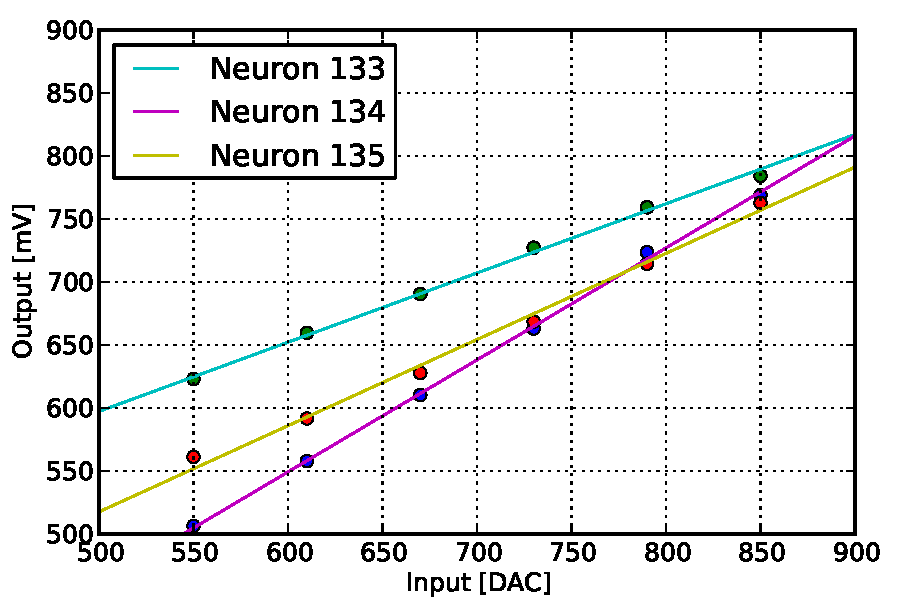
\includegraphics[width=0.5\textwidth]{figures/calib_example_lines}
  \caption{Calibration example.}
  \label{fig:calibration_example}
\end{figure}

Calibration steps are listed in the order in which they should be run.
For each parameter, you will find a description of what it does, how it is measured, what the calibration does to it and everything else that is worth noting.

The run\_calibration tool in the pycake/bin/ folder will calibrate all working parameters.
To configure the calibration, you have to edit parameters.py to match whatever you want to calibrate or measure.
There you can edit the calibrated ranges, step length and number of repetitions (which will increase accuracy but also linearly increase experiment time).
After calibration of a parameter, you should keep that variable within the range in which you calibrated -- outside of the range, the accuracy can decrease.

\subsection{Readout shift (21st parameter)}

\begin{figure}
  \centering
  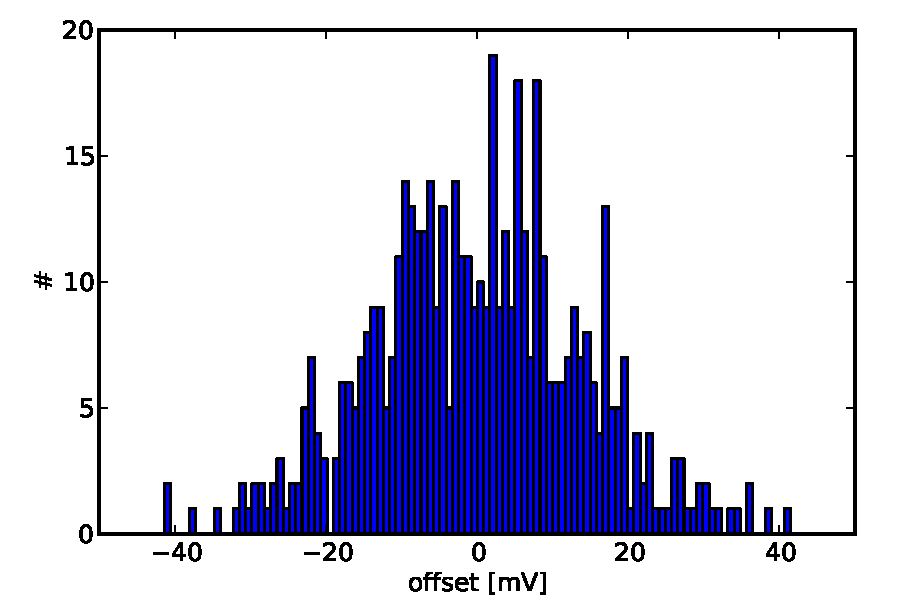
\includegraphics[width=0.5\textwidth]{figures/analog_readout_offset}
  \caption{Offset of analog readout buffer.}
  \label{fig:offset_analog}
\end{figure}

The neuron is connected to the readout amplifier via an operational amplifier.
This amplifier has a different offset for each neuron, which has to be measured in the first step.
For this purpose, we make use of the fact that one value of $V_\text{reset}$ is applied to a whole block of neurons, so that there should be no variation between this block.

\subsubsection*{Measurement}

First, $V_\text{reset}$ is measured for all neurons and averaged over each blocks.
This mean $V_\text{reset}$ is considered to be the "real" $V_\text{reset}$.
The readout shift is then calculated by taking each neuron's mean variation from that "real" value.
This shift is stored in calibtic as the 21st parameter.

\subsection{Reset Potential (\vreset)}



After a spike, the membrane potential is set to \vreset.
\begin{figure}
  \centering
  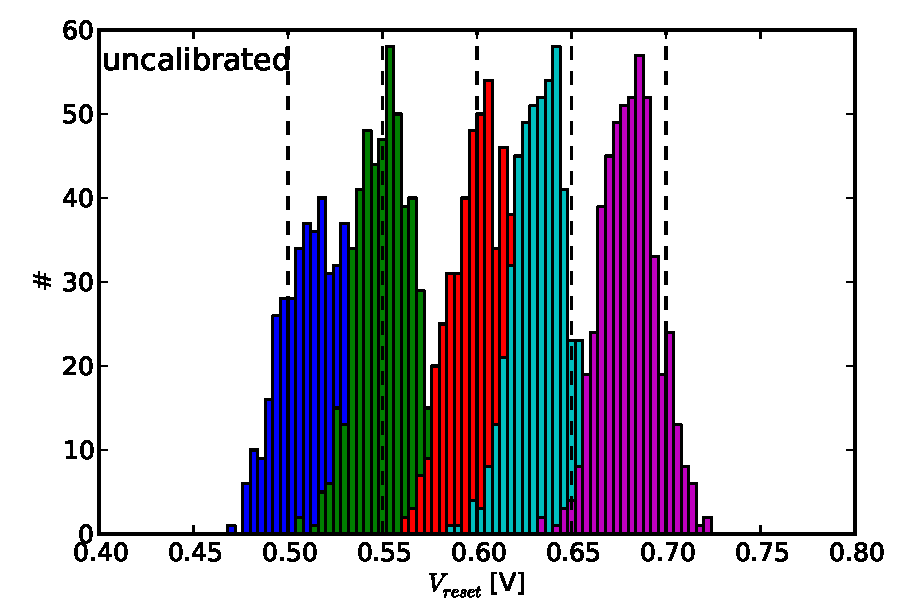
\includegraphics[width=0.5\textwidth]{figures/V_reset_uncalibrated}%
  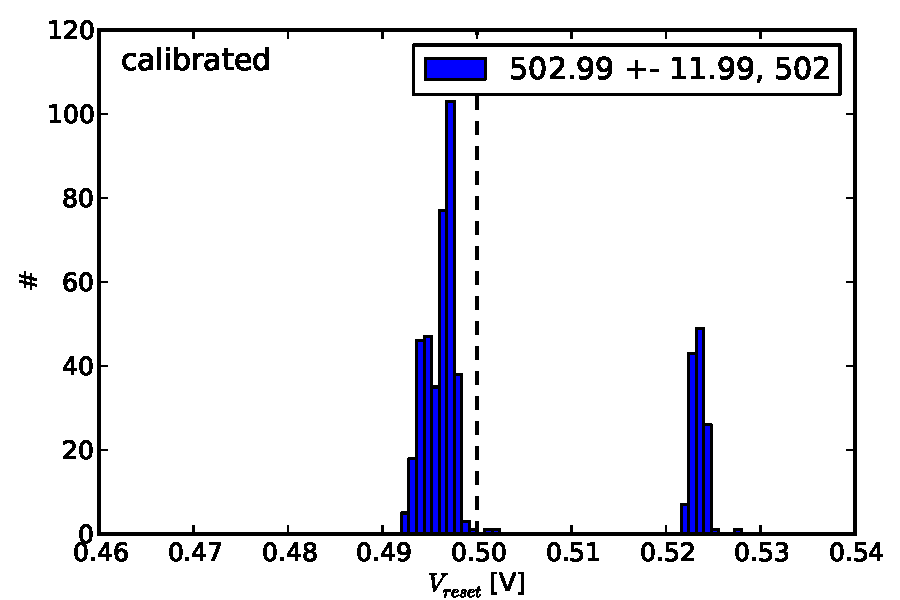
\includegraphics[width=0.5\textwidth]{figures/V_reset_calibrated}
  \caption{Uncalibrated (left) and calibrated (right) \vreset.}
  \label{fig:vreset_uncalib_calib}
\end{figure}
.
This parameter corresponds to the pyNN parameter \vreset.

Since this parameter is a shared parameter, it can not be set for each neuron individually but only for blocks of 128 neurons.
In this case, the calibration reduces block-to-block variation.

\subsubsection*{Measurement}
\vreset\ is measured by chosing a long \tauref\ time.
Then, the neuron is set to be always spiking. The value of the
membrane during the refractory period is averaged.

\subsection{Reversal Potentials (\esyni\ and \esynx)}

\esyni\ and \esynx\ are the synaptic reversal potentials. 
These voltages are applied at the $OTA_0$ in the synaptic input circuit (see \cref{figure:synapse}). 
Their pyNN-counterparts are e\_rev\_I and e\_rev\_E.

\begin{figure}
\centering
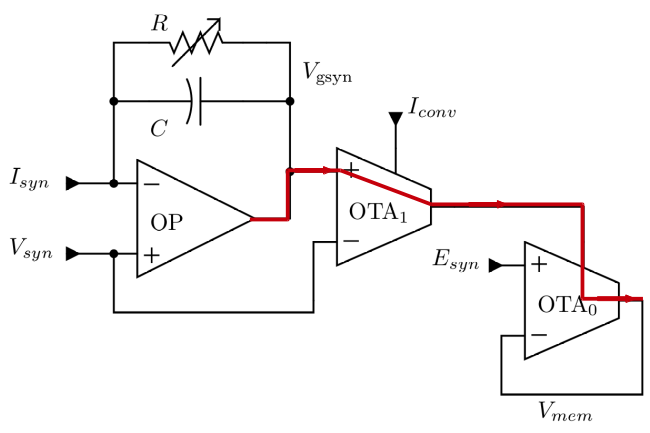
\includegraphics[width=0.5\textwidth]{figures/synin_dominik}
\caption{Synapse circuit. \esyn\ is applied to OTA0}
\label{figure:synapse}
\end{figure}

\subsubsection*{Measurement}

\begin{figure}
  \centering
  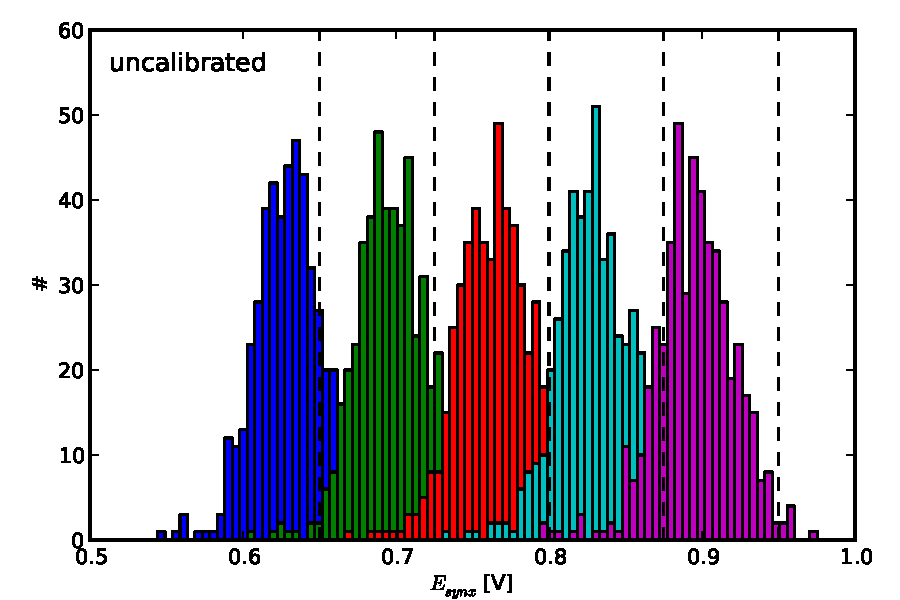
\includegraphics[width=0.5\textwidth]{figures/E_synx_uncalibrated_without_defects}%
  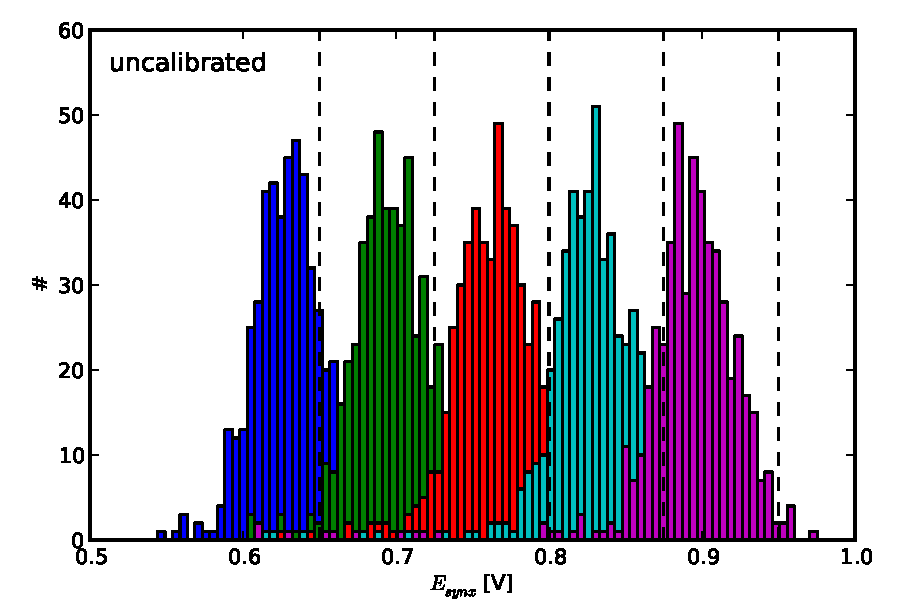
\includegraphics[width=0.5\textwidth]{figures/E_synx_uncalibrated_with_defects}
  \caption{\esyn\ calibration. Without (left) and with (right) inclusion of neurons flagged as not responsive to calibration protocol.}
  \label{fig:esyn_before_calibration}
\end{figure}

\begin{figure}
  \centering
  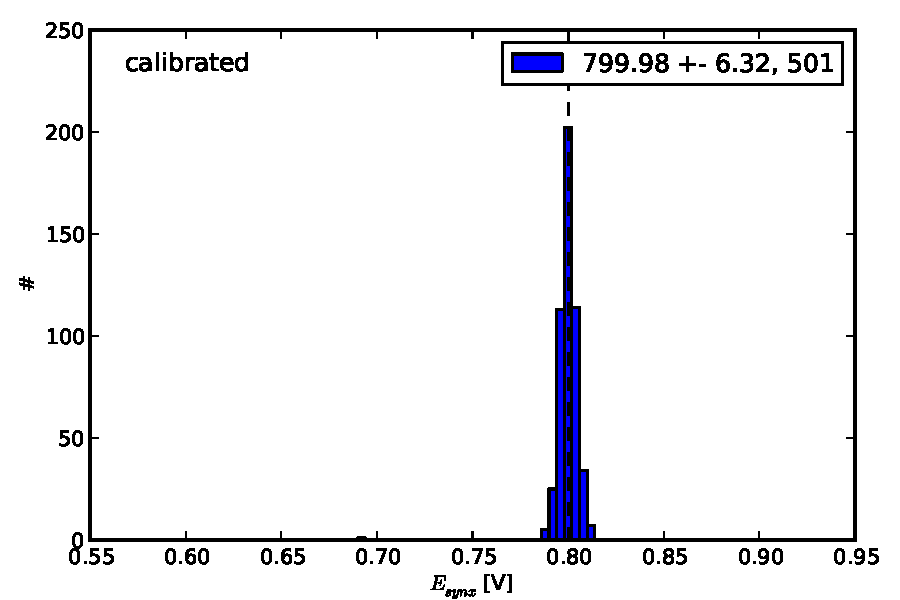
\includegraphics[width=0.5\textwidth]{figures/E_synx_calibrated_without_defects}%
  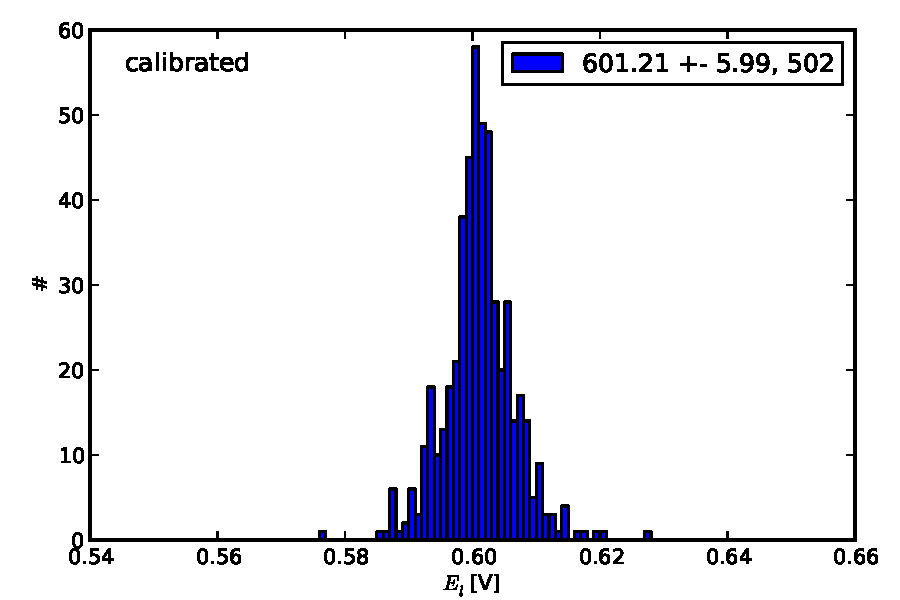
\includegraphics[width=0.5\textwidth]{figures/E_syni_calibrated_without_defects}
  \caption{\esynx\ and \esyni\ after calibration.}
  \label{fig:esyn_after_calibration}
\end{figure}

The synaptic reversal potentials are measured using leakage currents of the synaptic input circuit.
Since inhibitory and excitatory input circuits are identical, I will only describe the measurement once.

Ideally, when no spike input is present, there should be no leakage current through $OTA_0$.
However, due to imperfections in the manufacturing process, these leakages cannot be avoided.
Here, we make use of them by turning off all other conductances in the neuron circuit.
With the synaptic input being the only remaining conductance, the membrane potential will approach the synaptic reversal potential.
This can easily be measured with the ADC, thus giving an approximation of the reversal potential.

In addition, the background generators are used as input\ldots

\subsection{Leak Conductance (\igl)}

\begin{figure}
  \centering
  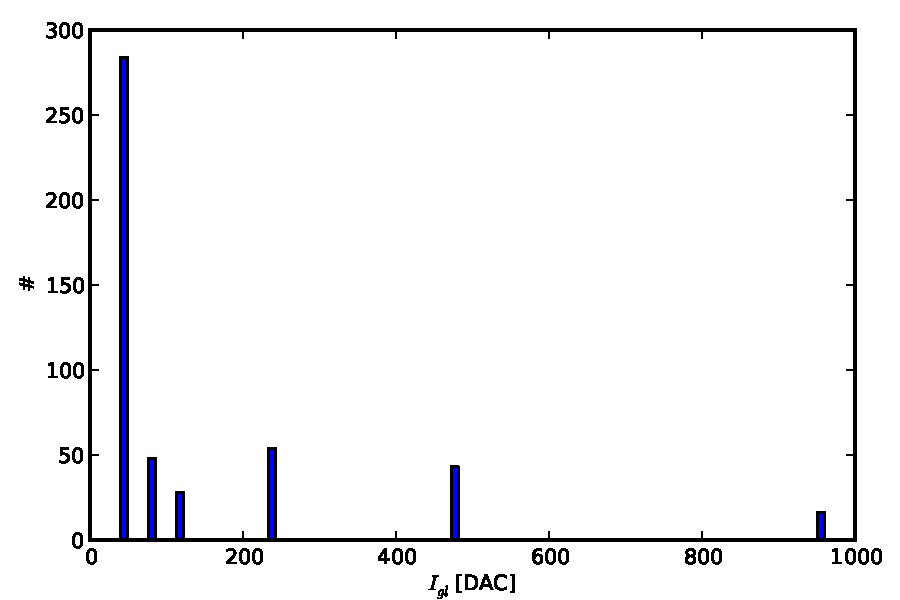
\includegraphics[width=0.5\textwidth]{figures/hist_I_gl}
  \caption{\igl}
  \label{fig:igl}
\end{figure}

Ideally, the leakage conductance is used to control the membrane time
constant. However, to maximize the effect of synaptic input, a small
conductance is beneficial. Therefore, a two dimensional scan of
\igl\ and \el\ is performed that finds the smallest
\igl\ for which the target membrane potential can be reached.

%\subsubsection*{Measurement}

\subsection{Synaptic Time Constant (\vsyntc)}

The value of the synaptic time constant has a strong effect on the PSP
height. Only in a small window, synaptic input can be observed at all,
see \cref{fig:v_syntc_calibration}.

\subsubsection*{Measurement}

\begin{figure}
  \centering
  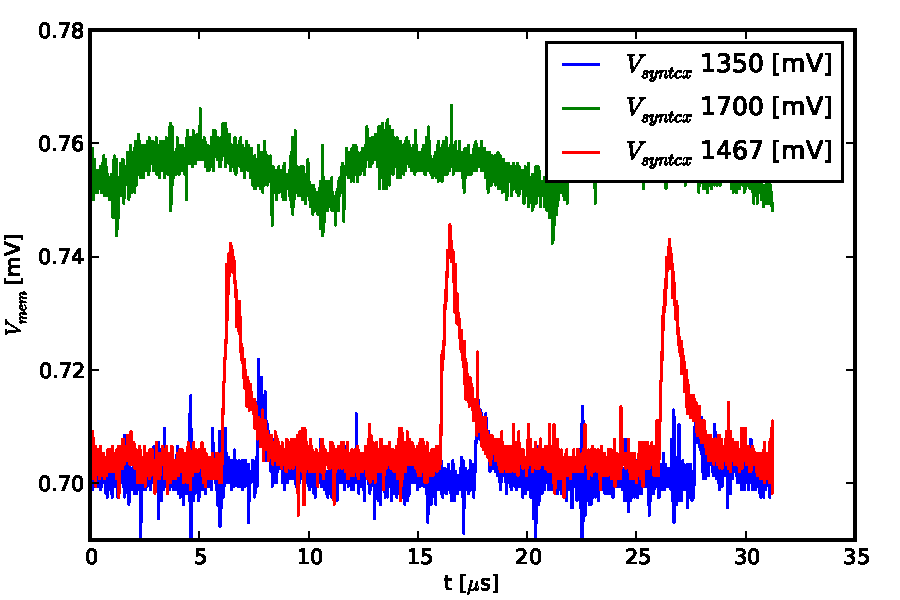
\includegraphics[width=0.5\textwidth]{figures/V_syntcx_trace}%
  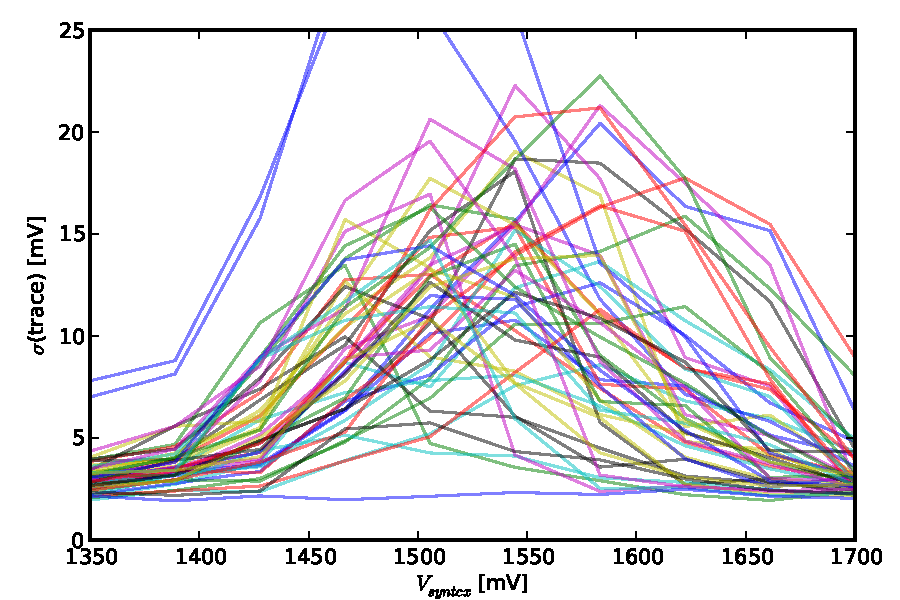
\includegraphics[width=0.5\textwidth]{figures/V_syntcx_scan}\\
  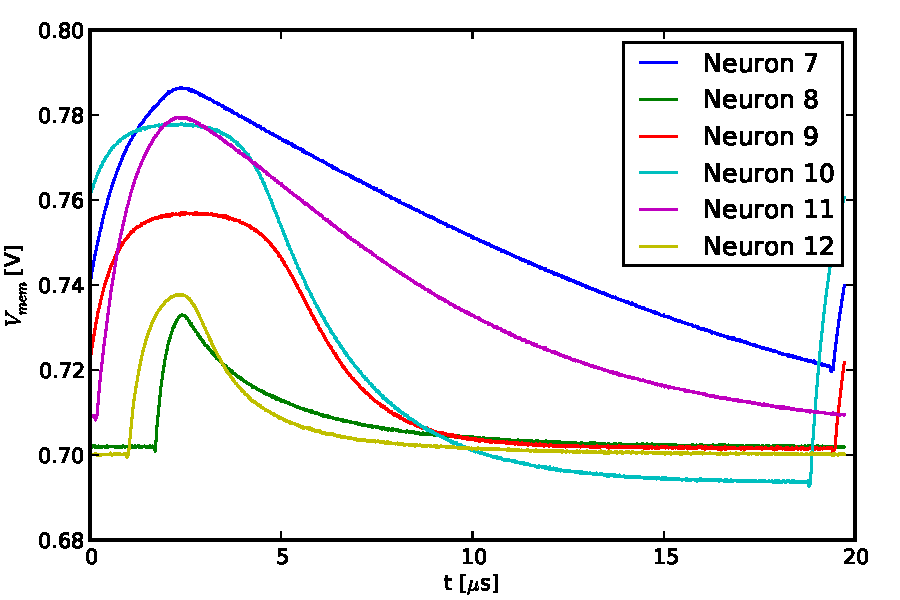
\includegraphics[width=0.5\textwidth]{figures/V_syntcx_psp_max_traces}
  \caption{\vsyntc\ calibration. Traces for different \vsyntcx\
    settings demonstrating the small range of operation. PSP heights
    as function of \vsyntcx. PSP shapes after picking the \vsyntcx\
    that maximizes the height.}
  \label{fig:v_syntc_calibration}
\end{figure}

The standard deviation, i.e.\ the spread, of the voltage trace is used
as a proxy for the PSP height. The value of synaptic time constant
that maximizes the spread is picked.

\subsection{Resting Potential (\el)}
\el\ is the membrane leakage potential that determines where the membrane potential should stay when no input is given at all.
It is applied at the leakage OTA (see \cref{figure:synapse}).
The corresponding pyNN parameter is the resting potential \vrest.

While calibrating, the synaptic reversal potentials are fixed and typically set
symmetrically around the target \el\ with a distance of \SI{100}{\milli\volt}.

\subsubsection*{Measurement}

\begin{figure}
  \centering
  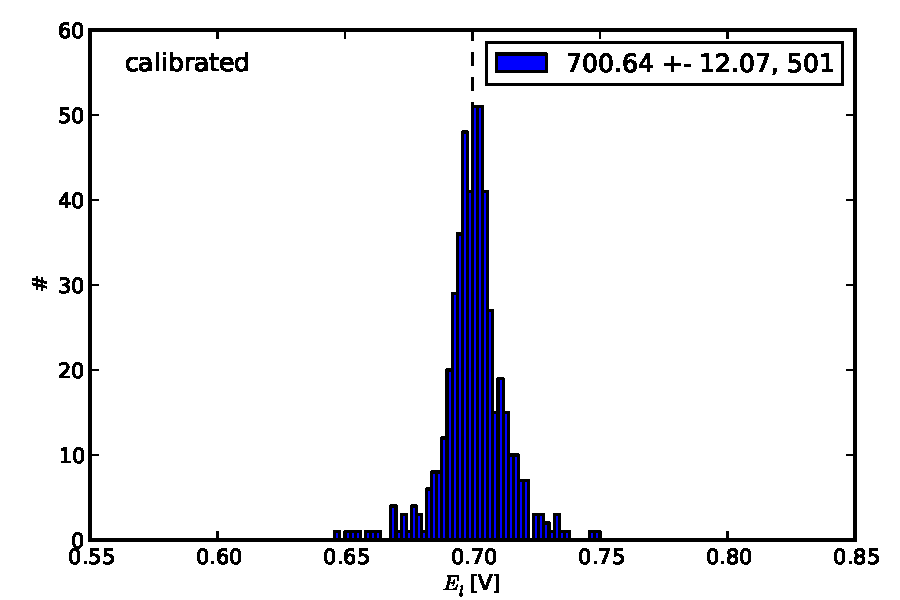
\includegraphics[width=0.5\textwidth]{figures/E_l_calibrated_without_defects}
  \caption{\el\ after calibration.}
  \label{fig:el_calibrated}
\end{figure}

\el\ is measured by turning on all conductances that will later be turned on while experiments are run.
That way, it is ensured that we calibrate an effective resting potential that balances the unwanted leakage currents.
Then, without any input, the membrane potential approaches a value which will be considered as \el.

\subsection{Threshold Potential (\vt)}
\vt\ is the voltage at which a spike is initiated.
This voltage corresponts to the pyNN parameter $V_{\text{thresh}}$ in a LIF model.

\subsubsection*{Measurement}

\begin{figure}
  \centering
  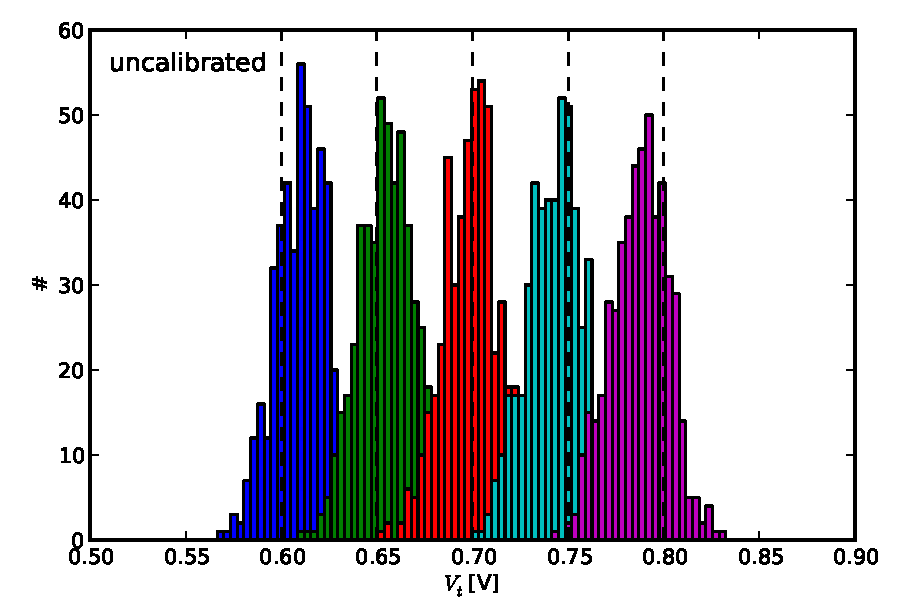
\includegraphics[width=0.5\textwidth]{figures/V_t_uncalibrated_without_defects}%
  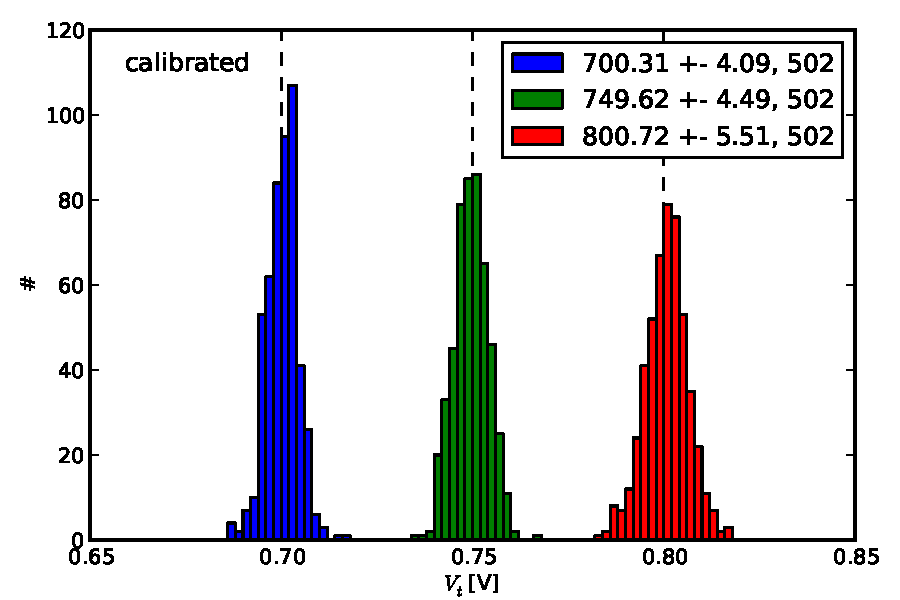
\includegraphics[width=0.5\textwidth]{figures/V_t_calibrated_without_defects}\\
  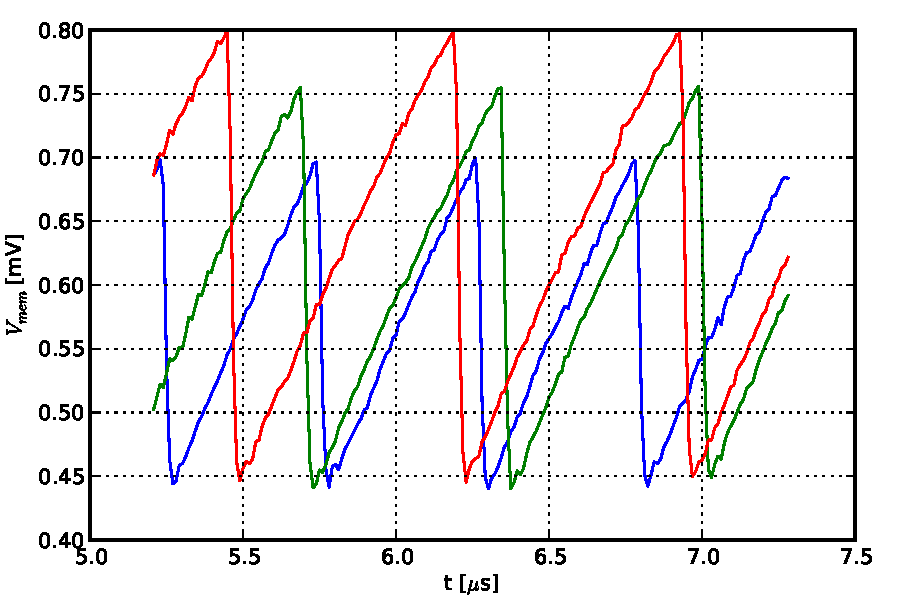
\includegraphics[width=0.5\textwidth]{figures/V_t_trace}
  \caption{\vt\ before (left) and after (right) calibration.}
  \label{fig:v_t_calibration}
\end{figure}

To measure \vt, the resting potential \el\ is set
above the threshold so that the neuron is spiking all the time.  Then,
the peaks of the trace are found and averaged, see \cref{fig:v_t_calibration}. This might
underestimate the threshold because the ADC might sample too early or
too late. However, relying on e.g.\ the maximum of the full trace
results in larger variations.

\subsection{Refractory Period (\ipl)}

\begin{figure}
  \centering
  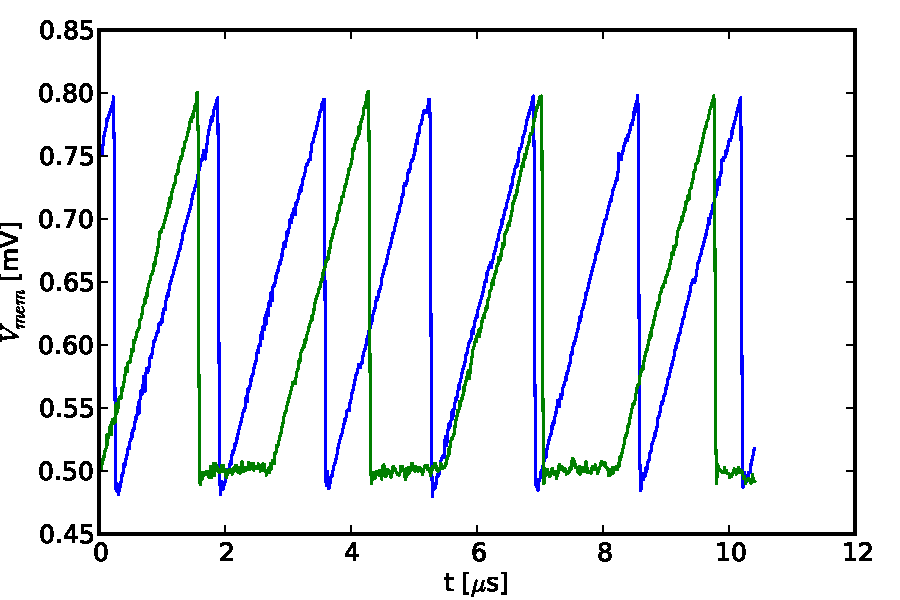
\includegraphics[width=0.5\textwidth]{figures/I_pl_trace}%
  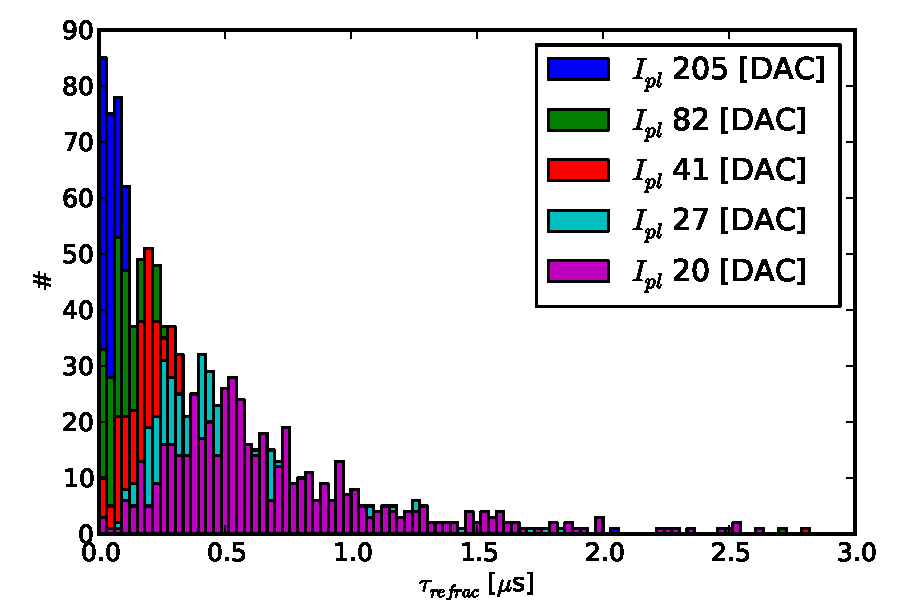
\includegraphics[width=0.5\textwidth]{figures/I_pl_hist}
  \caption{\ipl\ calibration.}
  \label{fig:tau_ref_calibration}
\end{figure}

The refractoy period \tauref\ determines how long a neuron stays at
\vreset\ after it elicited a spike, see \cref{fig:tau_ref_calibration}.

\subsubsection*{Measurement}

\tauref\ depends $\propto \frac{1}{\ipl}$.  First, \ipl\ is set very
high to achieve an approximately vanishing refractory period. With
this setting, the spike to spike time $\Delta s$ is
determined. Assuming no change in the spike to spike time, $\Delta s$
serves as reference that is subtracted for runs with increased
\tauref\ (decreased \ipl).

\end{document}
